\documentclass{css}
%\documentclass[english]{css}

\usepackage[dvips]{graphicx}
\usepackage{latexsym}

\def\|{\verb|}

\newcommand{\cssyear}[0]{2023}
\newcommand{\cssname}[0]{CSS 2023}
\newcommand{\cssversion}[0]{2023/06/01}
\newcommand{\cssemail}[0]{css2023-office@iwsec.org}

\begin{document}

%% 本文が和文の場合,タイトル・著者名・著者所属・概要は,和文・英文共に必須.
%% If you prepare this manuscript in English, there is no need to put Japanese metadata (title, author names, affiliations, abstract, and keywords) in it.

\title{Isolation Forestを用いた\\IoT向け異常検知手法に関する考察}
\etitle{A Study on Anomaly Detection Method \\for IoT using Isolation Forest}

\affiliate{XX}{東京工業大学 情報理工学院 数理・計算科学系\\
Department of Mathematical and Computing Sciences, School of Computing, Tokyo Institute of Technology}
\affiliate{YY}{東京工業大学 学術国際情報センター\\
Global Scientific Information and Computing Center}

%% メールアドレスは省略可能だが,代表者のメールアドレスは必須.
%% 姓名の間は半角スペースを入れること.

\author{菅田 大輔}{Daisuke Sugata}{XX}[sugata.d.aa@m.titech.ac.jp]
\author{石井 将大}{Masahiro Ishii}{YY}[mishii@gsic.titech.ac.jp]
\author{松浦 知史}{Satoshi Matsuura}{YY}[matsuura@gsic.titech.ac.jp]

%% the following is author command for english option.
%% at least one e-mail address is required.

%\author{Taro Joho}{XX}[taro.joho@xx.ac.jp]
%\author{Hanako Anzen}{XX, YY, ZZ}

\begin{abstract}
    本論文では, Isolation Forestを用いたIoT向け異常検知手法の改善を行った. この研究の背景には, IoT(Internet of Things)の普及があり, すべてのIoT機器のセキュリティ確保が重要な課題となっている. 本研究では, 専門的なセキュリティ対策が難しい家庭内ネットワークなどの小規模環境に着目し, 軽量で高速な異常検知システムの提案を目指した. AbuAlghanamらが提案したIsolation Forestを用いたIoT向けIDSは, その軽量性と高速性から今回の想定に適しているが, 二つの問題が存在する. 閾値を手動で設定する必要がある点と, 閾値による異常判定アルゴリズムの精度に限界がある点である. これらの課題を解決するため, 本研究では異常判定にロジスティック回帰を応用した判定アルゴリズムを提案する. 提案手法を二つのデータセットで実験した結果, 精度がそれぞれ82.1\%から90.7\%, 85.7\%から94.9\%に改善したことを確認した. 
\end{abstract}

%% キーワード (1--5単語) の記載は任意.

\begin{jkeyword}
Isolation Forest, IoT, IDS, 異常検知
\end{jkeyword}

\begin{eabstract}
    In this paper, we propose an improvement to the anomaly detection method for IoT using Isolation Forest. The background of this study lies in the widespread adoption of the Internet of Things (IoT), where ensuring the security of all IoT devices has become a critical issue. This research aims to propose a lightweight and fast anomaly detection system, particularly suited for small-scale environments such as home networks, where implementing specialized security measures is challenging. The IoT-oriented IDS using Isolation Forest proposed by AbuAlghanam et al. is suitable for this scenario due to its lightweight and fast nature. However, it has two major issues: the need for manual threshold setting and the limited accuracy of the anomaly detection algorithm based on these thresholds. To address these challenges, we propose a detection algorithm that applies logistic regression to anomaly detection. Experimental results on two datasets showed that the accuracy improved from 82.1\% to 90.7\% and from 85.7\% to 94.9\%, respectively.

\end{eabstract}

%% the following keyword part is optional and can be omitted.

\begin{ekeyword}
Isolation Forest, IoT, IDS, Anomaly Detection
\end{ekeyword}

%% if you use english opsion, you should put your English abstract in the abstract environment.
%% eabstract is not displayed in english mode.

\maketitle

\section{はじめに}
Isolation Forest(以下, IF)は, その計算効率の良さから異常検知に広く用いられている. 例えば, AbuAlghanamらはIoT向けのIDS(Intrusion Detection System)としてIFを用いた手法を提案している\cite{AbuAlghanam2023-sx}. しかし, AbuAlghanamらの手法には, 手動で閾値を設定する必要がある点や, 判定の組み合わせ方法における精度の限界といった課題が存在していた. 本研究では, これらの問題に対処するためにIFの異常判定にロジスティック回帰を応用し, AbuAlghanamらの研究手法の改善を行なった. 

この研究の背景として, IoT(Internet of Things)の急速な普及が挙げられる. 実際に2030年には約300億台ものデバイスが利用されると予測されており\cite{Vailshery2022}, すべてのIoT機器のセキュリティ確保が重要な課題となっている. 特に2016年のMirai型マルウェアによるDDoS攻撃はその必要性を浮き彫りにした\cite{8115504}.  家庭用のルーターやデジタルビデオレコーダーなどの管理不十分なデバイスがMirai型マルウェアに感染し, 一斉に特定のサーバーにアクセスを行うよう強制され, GitHub, Twitter, Reddit, Netflixなど, いくつかの有名ウェブサイトがアクセス不能になった.

公的機関や企業組織といった大規模な環境では, セキュリティの専門家が構築し運用するフレームワークによってIoT機器の安全性が確保されている. しかし, 先述した通りIoT機器は多くの場所で使用されており, 家庭内のネットワークなどの小さな組織の場合となると, これらを管理・運用するための人員リソースを確保することや, 高価なセキュリティシステムを導入することは困難である. そのため, 安価な計算機環境でも高速に動作するようなセキュリティシステムが求められている.

こうした背景から, 小規模な環境に適した IDS (Intrusion Detection System) の設計について考察する. 2章でIFのアルゴリズムの解説とIDSの概要を説明する. 3章で従来のIFを用いた異常検知手法の問題点を整理し, これらの問題を解決する提案手法について述べる. 5章では, UNSW-NB15とNSL-KDDの2つのデータセットを用いて, 提案手法の有効性を評価した.

\section{研究方法}

\subsection{Isolation Forestの説明}

Isolation Forest(以下, IF)は, Liuらが提案した\cite{Liu2008-bc}外れ値を効率的に検出するためのアルゴリズムである. この手法は異常データの数が少なく, 他の正常データから離れて存在するという特性に基づいて設計されている. データをランダムに分割していく過程で異常データは正常データに比べて相対的に早く孤立するため, データが孤立するまでに必要な分割回数に着目することで, 異常データを検出できる. IFの実行は以下のステップに分かれる. 

\subsubsection{データの分割}

IFは, ランダムに選んだ特徴量を基にデータを分割する. 具体的には, 選んだ特徴量のランダムな値を閾値として使用し, その閾値より大きいグループと小さいグループにデータを二分割する. この分割を全てのデータが孤立するまで繰り返し行い, 一つの決定木($iTree$)を作成する. このプロセスが終了したら, 複数の決定木を構築する. 

\subsubsection{異常スコアの算出}

異常スコアは, データ点が生成された$iTree$の枝をたどって到達するまでのパス長に基づいて計算される. パス長が短いほど, そのデータ点は異常である可能性が高い. 異常スコア$V(x,n)$の計算式は式\ref{eq:anomaly_score}の通りである. 


\begin{equation}
    V(x, n) = 2^{-\frac{E(h(x))}{c(n)}}
    \label{eq:anomaly_score}
\end{equation}

ここで$E(h(x))$はデータ点$x$の平均パス長$c(n)$はデータセットのサイズ$n$に依存する調整用の定数である. 

\subsubsection{異常判定}
計算された異常スコアを使用して, 異常検知を行う. scikit-learnのライブラリを用いた実装では, パラメータ contaminationで閾値を設定する. contaminationは float 型で $(0, 0.5]$ の間の値をとり, データセット内で異常と見なすデータの割合を指定する. このパラメータに基づいて, トレーニングデータ内で指定された割合に相当するスコアの値が閾値として設定される. この閾値を超えるスコアを持つデータは異常と判定される. 


\subsection{AbuAlghanamらの提案手法}
本研究では, 小規模環境でも軽量に動作する,AbAlghanamらが提案したIFを用いたIDSの手法\cite{AbuAlghanam2023-sx}に注目し,彼らの研究を大いに参考にしIDSの設計を行った. 

\subsection{全体の設計}
AbuAlghanamらが提案したIDSの設計\cite{AbuAlghanam2023-sx}は,図\ref{fig:IDS}に示すように, データの前処理, 特徴量選択, 異常判定の3つのステップで構成される. 

\begin{figure}[ht]
    \centering
    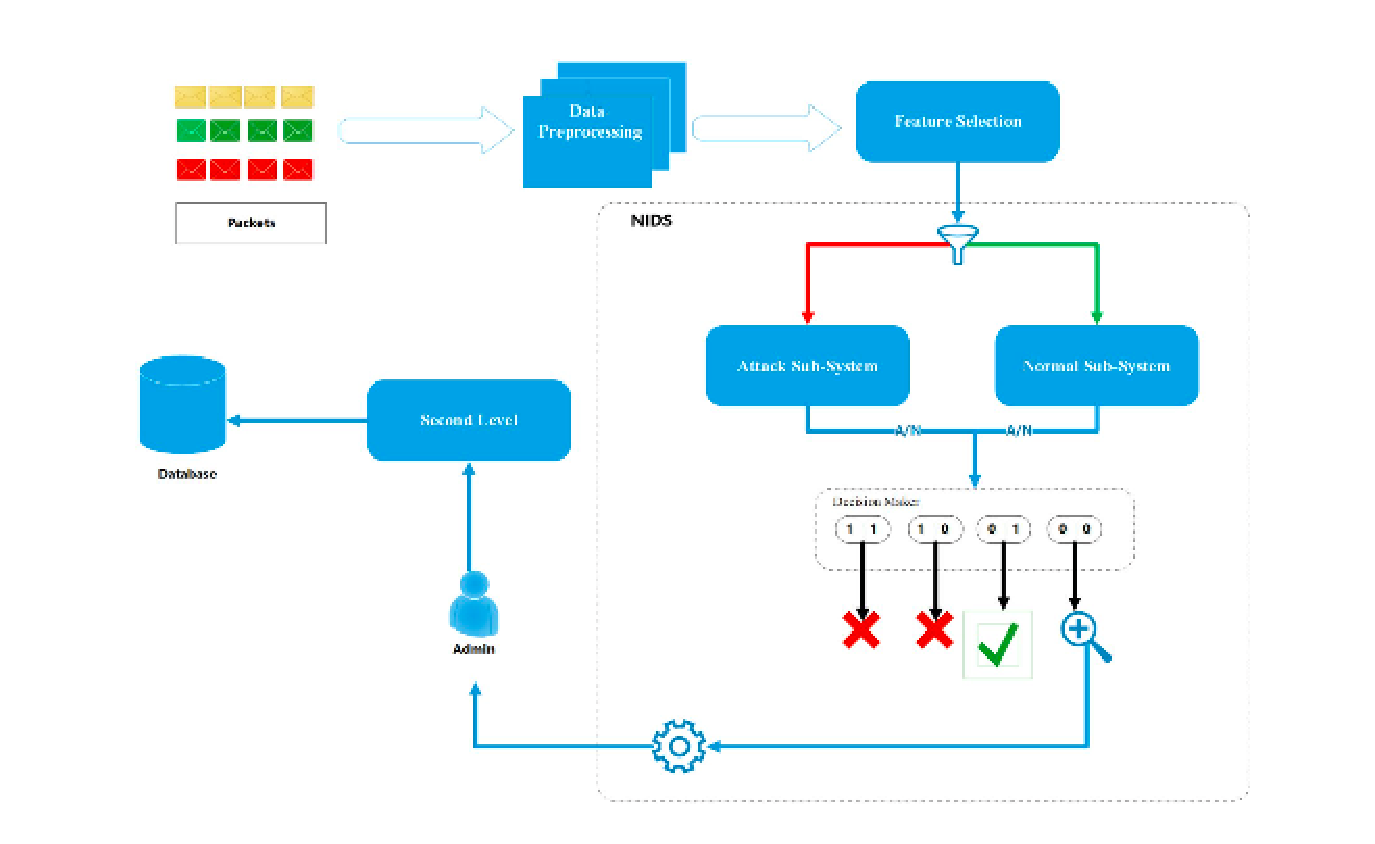
\includegraphics[width=0.9\linewidth]{pictures/eps/system.eps}
    \caption{AbuAlghanamらのIDSの全体の設計(出典:\cite{AbuAlghanam2023-sx})}
    \label{fig:IDS}
\end{figure}

\subsubsection{データの前処理}

はじめにタイムスタンプやIPアドレスといった, IFで使用しない特徴量を削除する. 次に, IFが数値データのみを入力として受け付けるため, カテゴリカルデータを数値データに変換する. この変換にはone-hotエンコーディングを利用し, 異なるカテゴリの特徴を個別の数値特徴として表現する. さらに, データセットは攻撃データと正常データに事前に分割され, それぞれ別のデータセットとして扱われる. 

\subsubsection{特徴量選択}
AbuAlghanamらの研究では, 特徴量選択の手法として主成分分析(PCA)および特徴重要度(FI)法を使用した\cite{AbuAlghanam2023-sx}との記述があったが, 具体的な手法については記載されていなかった. 本研究では特徴量のRandom Forestアルゴリズムを用いて重要度を計算し, 設定された閾値を超える特徴量のみを選択した. 

\subsubsection{異常判定}
AbuAlghanamらの手法では, データを攻撃通信と正常通信の2つに分割し, それぞれに対してIFのトレーニングを行う. この2つのトレーニングされたIFをサブシステムと呼ぶ. 2つのサブシステムは各データに対して異常スコアを算出する. 異常スコアはどの程度データが異常であるかを定量的に表す指標である. その後, 設定した閾値を超える異常スコアを持つデータをAnomalyと判定する. AbuAlghanamらの手法では, 最終的な判定は2つのサブシステムの判定を表\ref{tab:combination}のように組み合わせることで行われる. 本研究のIDSでは, この判定の組み合わせ手法の代わりにロジスティック回帰を用いた判定アルゴリズムを採用した. 

\begin{table}[ht]
    \caption{AbuAlghanamらの判定組み合わせ手法}
    \centering
    \footnotesize
    \begin{tabular}{ccc}
        \hline\hline
        正常サブシステム & 攻撃サブシステム & 判定結果\\
        \hline
        Normal & Anomaly & Normal \\
        Anomaly & Normal & Anomaly \\
        Normal & Normal & Anomaly \\
        Anomaly & Anomaly & Unknown \\
        \hline
    \end{tabular}
    \label{tab:combination}
\end{table}


\section{問題点の整理}
まず, IFを異常検知手法として適用する際にどのような問題があるのかを明らかにするため, 事前実験を行った.はじめにデモデータを使用してIFの挙動を確認し,その考察をもとに特徴量選択手法の提案を行なった.また, AbuAlghanamらの提案したIFを用いた異常検知手法\cite{AbuAlghanam2023-sx}の問題点を整理した. 

\subsection{ノイズ特徴量が混入すると精度が悪化する問題}
使用するデモデータは, (2.5, 2.5)と(-2.5, -2.5)を中心とした正常データ群と, 10から-10の範囲に一様に分布した異常データ群からなる.二次元の場合のデモデータを図\ref{fig:demodata}に示す.

\begin{figure}[ht]
    \centering
    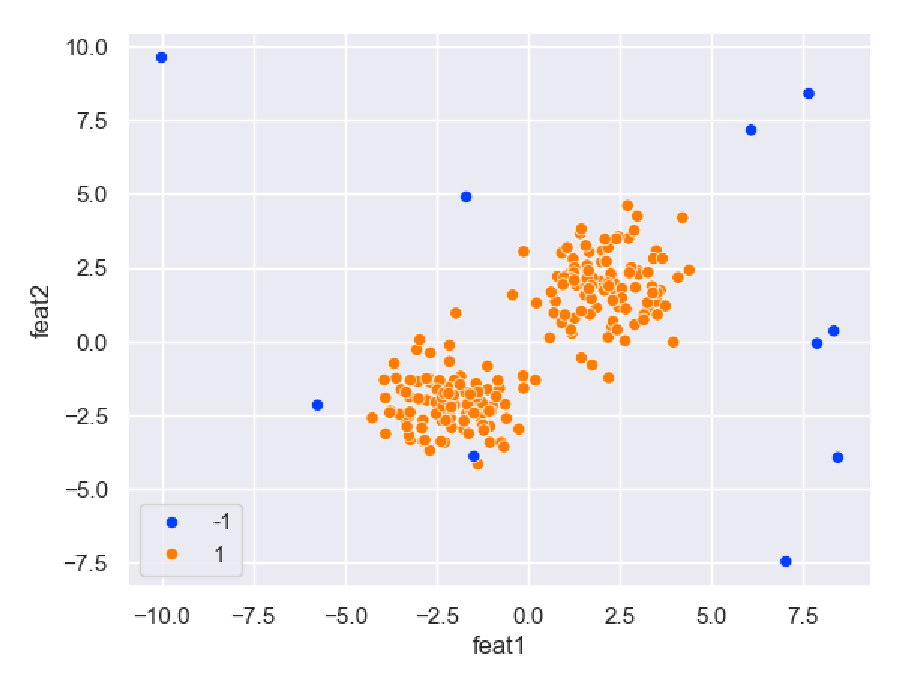
\includegraphics[width=0.9\linewidth]{pictures/eps/demodata.eps}
    \caption{デモデータの2次元グラフ}
    \label{fig:demodata}
\end{figure}

\subsubsection{特徴量数と精度の関係}
はじめに, デモデータと特徴量数の関係を調査した.図\ref{fig:dim_vs_accu}に示すように, 特徴量数が増えるにつれて, 異常検知の精度が単調に向上することがわかった.また, 精度ののびは増加に反比例して緩やかになっていることもわかる. ゆえに, IFは目標とする精度に対して十分な特徴量数が存在すると言える. 

\begin{figure}[ht]
    \centering
    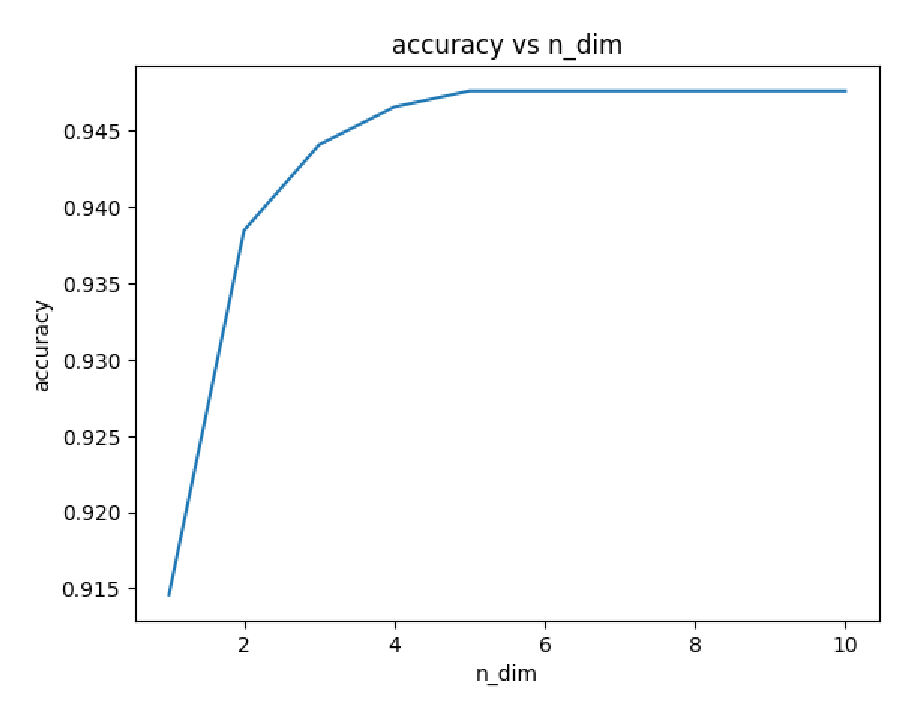
\includegraphics[width=0.9\linewidth]{pictures/eps/dim_vs_accu.eps}
    \caption{判定に有効な特徴量数とIFの精度の関係}
    \label{fig:dim_vs_accu}
\end{figure}

\subsubsection{ノイズ特徴量の影響}
続いて, デモデータにノイズ特徴量を含めたときの精度の悪化について調査した. パケット通信を監視して得られたデータセットの全ての特徴が, 異常検知に有効なわけではない. IFは特徴量同士の重みづけを行わないため, これらの判定に有効でない特徴量が混ざると精度が低下すると考えられる. そこで, デモデータにノイズ特徴量を含めていき, 精度の変化を調査した. 結果は図\ref{fig:noise_accu}に示すように, ノイズとなる特徴量が混ざると精度が低下することがわかった. また, 今回の実験の場合だと, ノイズ特徴量が判定に有効な特徴量数の2倍以上になると, 精度が急激に低下することがわかった. 

\begin{figure}[ht]
    \centering
    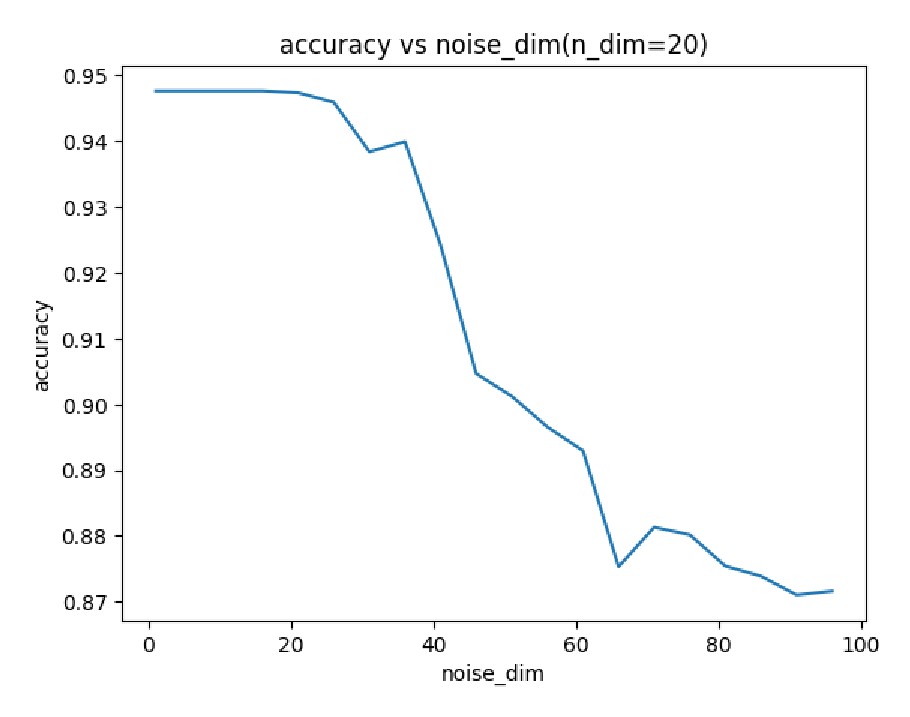
\includegraphics[width=0.9\linewidth]{pictures/eps/noise_accu.eps}
    \caption{ノイズ特徴量の精度に対する影響}
    \label{fig:noise_accu}
\end{figure}

\subsubsection{重要度に基づいたノイズ特徴量の除去}
前節の実験から, データセットからノイズとなる特徴量を取り除くことが重要であると考えられる. ところで, IFはツリーベースの異常検知手法である. そこで, 同じくツリーベースのRandam Forestから特徴の重要度を参照すれば, ノイズとなる特徴量を取り除けるのではないかと考えた. 図\ref{fig:select_noise}は, Random Forestで算出した特徴量の重要度を表している. このグラフは, ノイズ特徴量を判別できていることがわかる. そして, 実際にノイズ特徴量を取り除いた場合の精度を調査したところ, 精度は0.872\%から0.945\%まで向上した. この結果から, Feature Importanceによる特徴量選択手法は精度の向上に有効ではないかと考えた. 

\begin{figure}[ht]
    \centering
    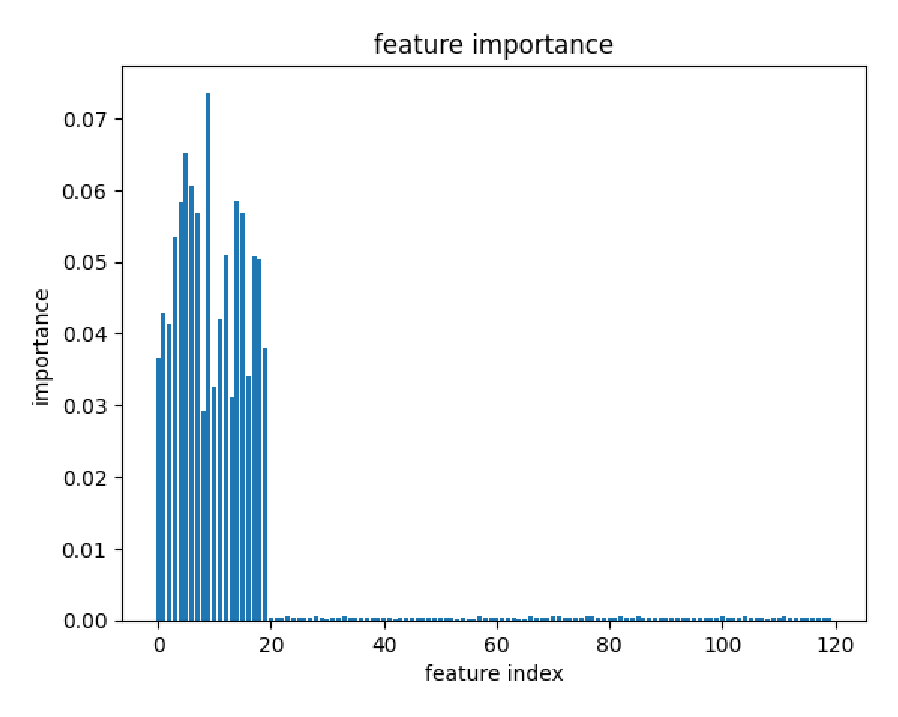
\includegraphics[width=0.9\linewidth]{pictures/eps/select_noise.eps}
    \caption{Random Forestで算出した特徴量の重要度}
    \label{fig:select_noise}
\end{figure}

\subsection{異常検知の境界線の問題}
AbuAlghanamらが提案したIFを用いた異常検知手法\cite{AbuAlghanam2023-sx}では, 2つのサブシステムが異常スコアを算出し, それが閾値を超えたデータを異常と判定する. そして, この2つの判定を表\ref{tab:combination}のように組み合わせて最終的な判定を行っている. しかし, この手法は, 以下の2つの問題を抱えている. 

\begin{itemize}
    \item 各サブシステムの異常スコアの閾値を手動で設定する必要があること. 
    \item 異常判定の境界線が垂直であるため, 異常スコアの分布によっては誤判定が多くなること. 
\end{itemize}

実際に異常スコアの分布を調査したところ, 図\ref{fig:UNSW-NB151}と図\ref{fig:NSL-KDD1}で示されるように, 異常データと正常データの境界線は対角方向になっている. 

\begin{figure}[ht]
    \centering
    \begin{minipage}{0.9\linewidth}
        \centering
        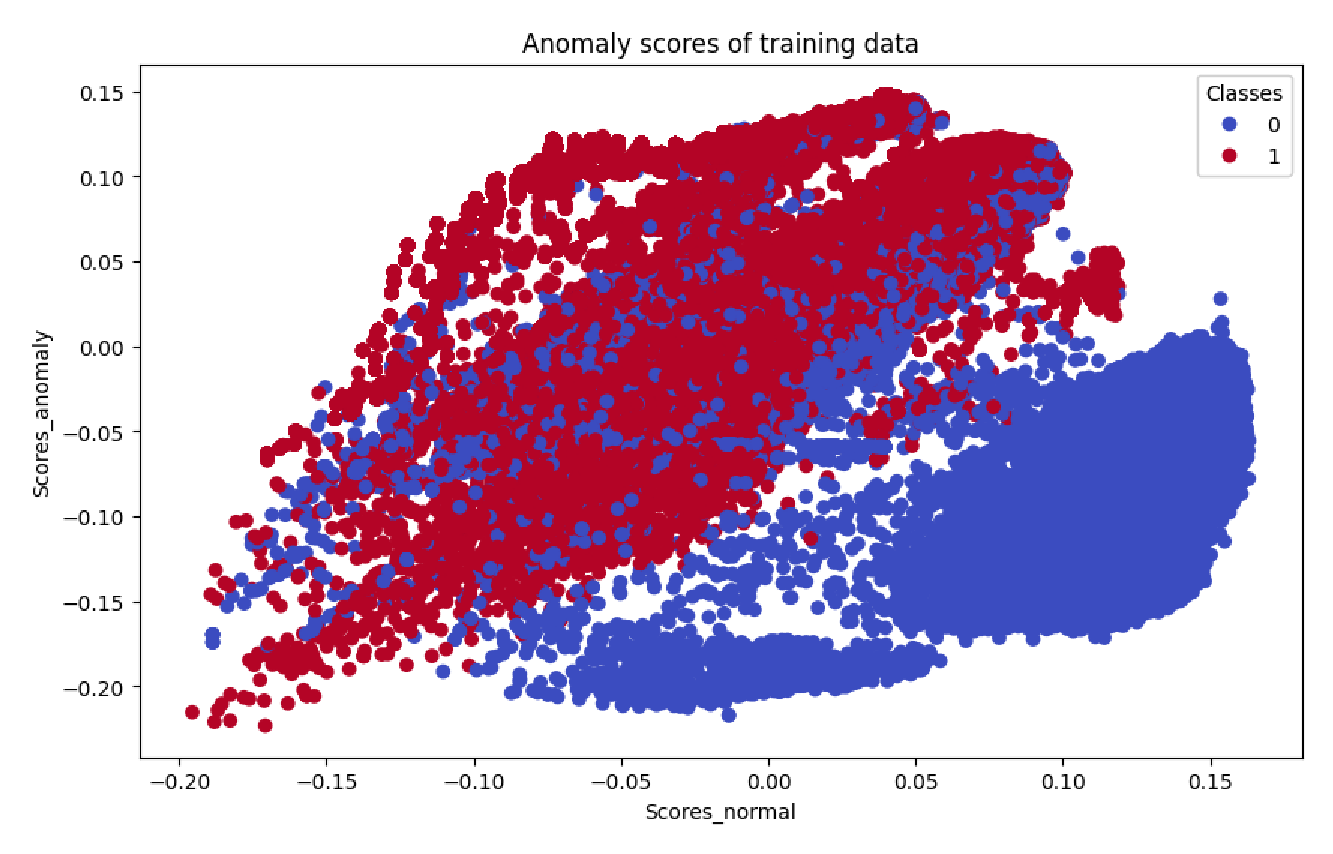
\includegraphics[width=\linewidth]{pictures/eps/UNSW-NB151.eps}
        \caption{UNSW-NB15における訓練データの異常スコア分布}
        \label{fig:UNSW-NB151}
    \end{minipage}
    \vfill{}
    \begin{minipage}{0.9\linewidth}
        \centering
        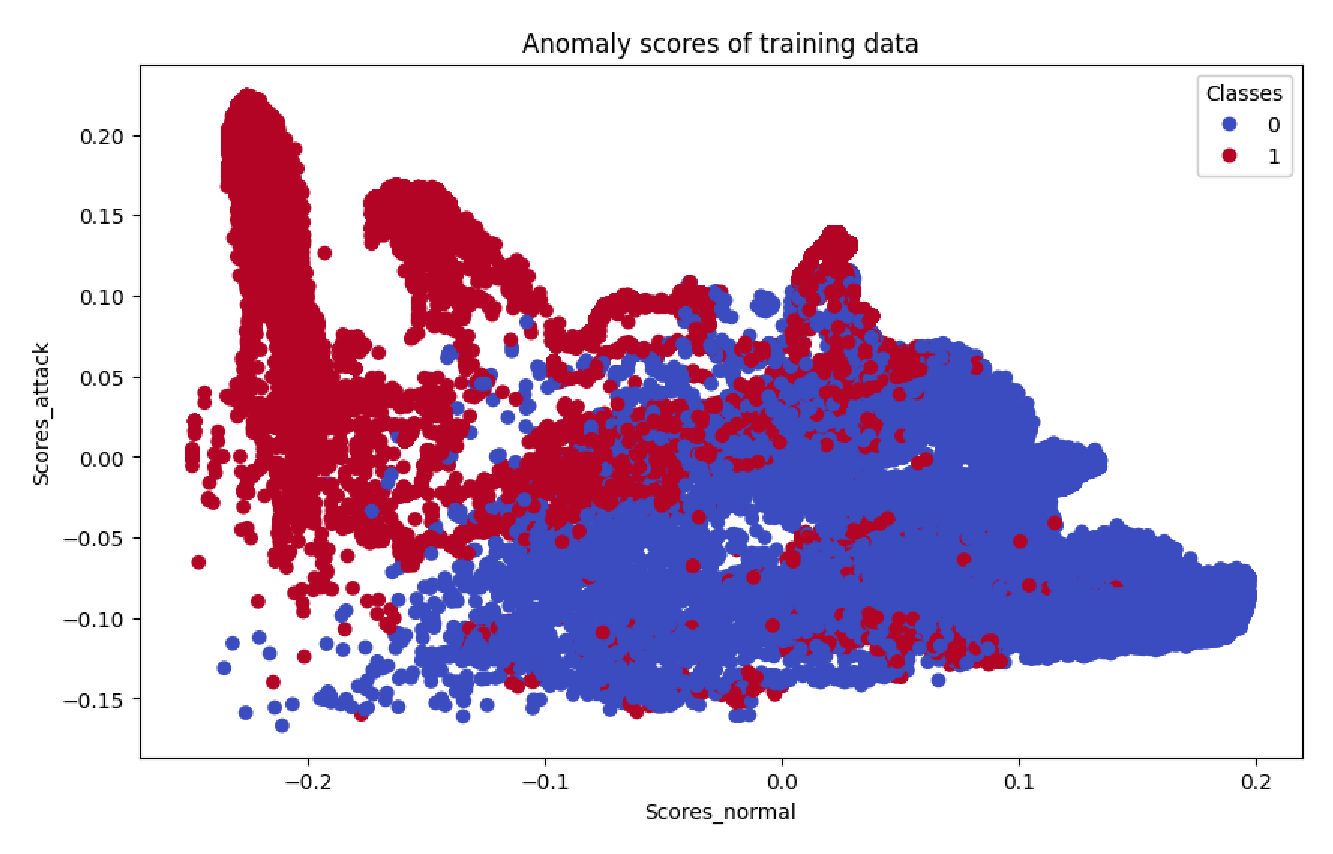
\includegraphics[width=\linewidth]{pictures/eps/NSL-KDD1.eps}
        \caption{NSL-KDDにおける訓練データの異常スコア分布}
        \label{fig:NSL-KDD1}
    \end{minipage}
\end{figure}

このような場合, AbuAlghanamらの手法\cite{AbuAlghanam2023-sx}のように, 垂直に分割しては誤検知が多く発生してしまう問題がある. 図\ref{fig:UNSW-NB152}と図\ref{fig:NSL-KDD2}は, AbuAlghanamらの手法による異常判定結果を示しているが, 垂直に分割する手法では, 異常データが多く誤検知されていることがわかる. 

\begin{figure}[ht]
    \centering
    \begin{minipage}{0.9\linewidth}
        \centering
        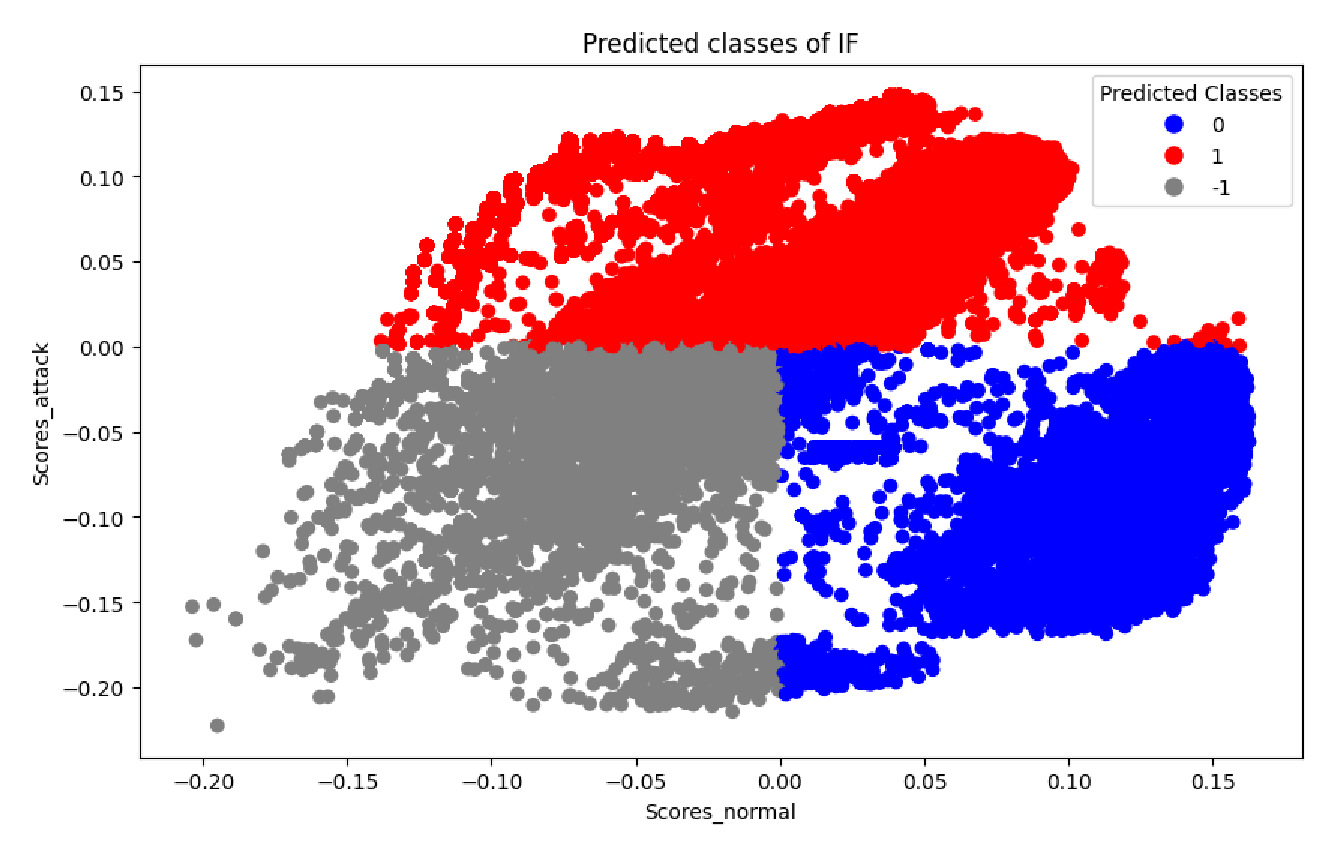
\includegraphics[width=\linewidth]{pictures/eps/UNSW-NB152.eps}
        \caption{UNSW-NB15におけるAbuAlghanamらの判定手法}
        \label{fig:UNSW-NB152}
    \end{minipage}
    \vfill{} 
    \begin{minipage}{0.9\linewidth}
        \centering
        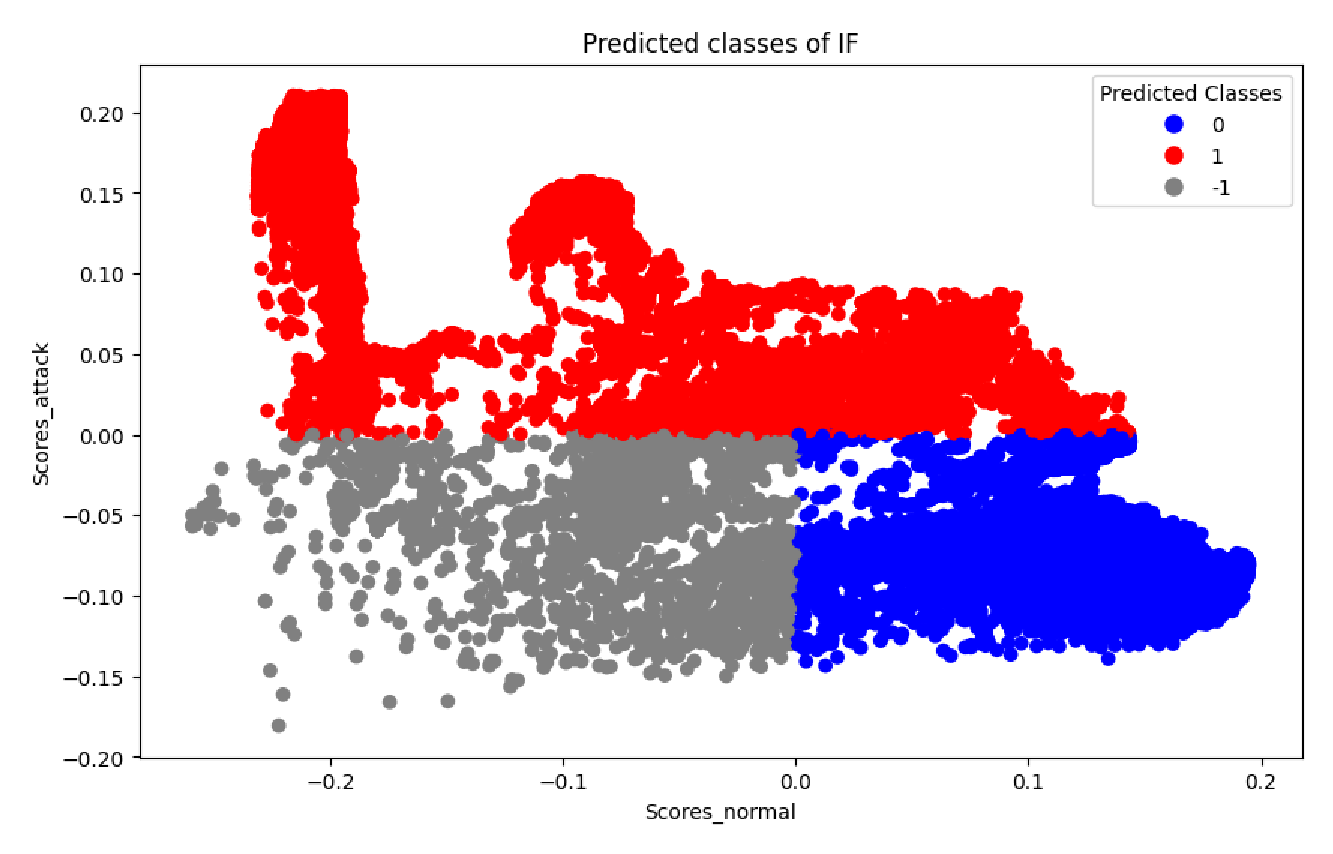
\includegraphics[width=\linewidth]{pictures/eps/NSL-KDD2.eps}
        \caption{NSL-KDDにおけるAbuAlghanamらの判定手法}
        \label{fig:NSL-KDD2}
    \end{minipage}
\end{figure}

この問題を解決するために, ロジスティック回帰を用いて異常判定の境界線を斜めに設定する手法を4章で提案する. 

\section{提案手法}
3章で述べた, 以下の2つの問題
\begin{itemize}
    \item ノイズ特徴量が精度に悪影響を及ぼす問題
    \item 異常検知の境界線の設定の問題
\end{itemize}
を解決するために, 以下の2つの提案を行った. 

一つは, ノイズ特徴量を取り除くための特徴量選択手法の提案である. もう一つは, 異常検知の境界線が斜めに分布する場合にも適切な判定ができるよう, ロジスティック回帰を用いて境界を決定する手法の提案である. 

\subsection{特徴量選択手法の提案}   
本手法の疑似コードは表\ref{tab:feature_selection}の通りである. まず, Random Forestを用いて特徴量の重要度を算出する. 次に, 特徴量の重要度の上位10\%を選択し, 新しいデータセットを作成する. 実装には, scikit-learnのライブラリを用いた\cite{scikit-learn}. 

\begin{table}[h!]
    \centering
    \caption{特徴量選択手法の擬似コード}
    \begin{tabular}{|l|}
    \hline
    \# Load training data \\
       \ \ \ \ data, labels = load\_data() \\ 
    \# Initialize Random Forest model \\
       \ \ \ \ model = RandomForest() \\ 
    \# Train the model \\
       \ \ \ \ model.fit(data, labels) \\ 
    \# Calculate feature importances \\
       \ \ \ \ feature\_importances = model.feature\_importances\_ \\ 
    \# Select top 10\% features \\
       \ \ \ \ threshold = np.percentile(feature\_importances, 90) \\
       \ \ \ \ selected\_features = feature\_importances $>$ threshold \\ 
    \# Create a new dataset with selected features \\
       \ \ \ \ new\_data = data[:, selected\_features] \\ \hline
    \end{tabular}
    \label{tab:feature_selection}
\end{table}


\subsection{ロジスティック回帰を適用した異常判定手法}
はじめに, 2つのサブシステムで訓練データの異常スコアを算出する. 次に, これらの異常スコアと訓練データのラベルを入力としてロジスティック回帰をトレーニングする. そして, テストデータの異常スコアを入力としてロジスティック回帰を適用し, 異常判定を行う. 疑似コードは表\ref{tab:logistic_regression}の通りである. ロジスティック回帰のパラメータは設定しておらず, scikit-learnのライブラリを用いて実装した. 

\begin{table}[h!]
    \centering
    \caption{ロジスティック回帰を適用した異常判定手法の擬似コード}
    \begin{tabular}{|l|}
    \hline
    \# Calculate anomaly scores \\
       \ \ \ \ score1 = sub1.predict(train\_data) \\
       \ \ \ \ score2 = sub2.predict(train\_data) \\ 
    \# Prepare training data \\
       \ \ \ \ X\_train = np.column\_stack((score1, score2)) \\
       \ \ \ \ y\_train = labels \\ 
    \# Train logistic regression \\
       \ \ \ \ clf = LogisticRegression() \\
       \ \ \ \ clf.fit(X\_train, y\_train) \\ 
    \# Apply to test data \\
       \ \ \ \ test\_score1 = sub1.predict(test\_data) \\
       \ \ \ \ test\_score2 = sub2.predict(test\_data) \\
       \ \ \ \ X\_test = np.column\_stack((test\_score1, test\_score2)) \\
       \ \ \ \ preds = clf.predict(X\_test) \\ 
    \hline
    \end{tabular}
    \label{tab:logistic_regression}
\end{table}


\section{結果と考察}

\subsection{比較するアルゴリズム}

本研究では, 以下の2つの比較を行った. 
特徴量選択手法の効果の比較を行うため, 特徴量選択を行わなかった場合と, Random Forestを用いた特徴量選択手法を用いた場合の結果を比較する. また, 判定の組み合わせアルゴリズムの比較には, AbuAlghanamらの2つのサブシステムの判定を組み合わせて検知を行う手法\cite{AbuAlghanam2023-sx}と, ロジスティック回帰を用いて判定を行う手法の結果を比較した. 

\begin{enumerate}
    \item \textbf{特徴量エンジニアリングの比較}
        \begin{itemize}
            \item 特徴量選択なし
            \item Random Forestを用いた特徴量選択手法
        \end{itemize}
    \item \textbf{判定の組み合わせアルゴリズムの比較}
        \begin{itemize}
            \item AbuAlghanamらの判定手法\cite{AbuAlghanam2023-sx}
            \item ロジスティック回帰を用いて判定
        \end{itemize}
\end{enumerate}

\subsubsection{実験環境}

実験はMac Book Pro 2017 2.3GHz Intel Core i5, 8GB RAMで行った. また, 実験に用いたプログラムはPython3.10.4で実装した. Isolation ForestやRandom Forestの実装には, scikit-learnのライブラリを用いた\cite{scikit-learn}. 

\subsubsection{データセット}
本実験では, 以下の2つのデータセットを用いた. 表\ref{tab:data1}にこれらのデータセットの概要を示す. 実験の際は, scikit-learnライブラリのtrain-test-split関数を用いて, これらのデータセットをトレーニングデータとテストデータに7:3に分割し評価を行った. 

\begin{enumerate}
    \item \textbf{NSL-KDD}\\
        異常検知や機械学習の分野で標準的なベンチマークデータセットとして広く利用されてきたKDDCUP99\cite{KDDCUP99}の問題点を解決するために, Tavallaeeらによって提案されたデータセットであり, データの冗長性や攻撃データの割合を調整したもの\cite{Tavallaee2009-we}. 
    \item \textbf{UNSW-NB15}\\
        既存のデータセットの問題点を解決し, 現代のネットワークトラフィックを包括的に反映するために, MoustafaとSlayによって作成されたデータセット\cite{Moustafa2015-cg}. 
\end{enumerate}

\begin{table}[h]
    \centering
    \caption{データセットの概要}\label{tab:data1}
    \begin{tabular}{lcc}
    \hline\hline
    No & NSL-KDD & UNSW-NB15 \\
    \hline
    データ数 & 125,972 & 175,341 \\
    正常データ数 & 67,343 & 56,000 \\
    攻撃データ数 & 58,629 & 119,341 \\
    特徴量数 & 43 & 45 \\
    エンコード後の特徴量数 & 124 & 198 \\
    \hline
    \end{tabular}
\end{table}

\subsubsection{評価指標}
本研究では, 以下の2つの評価指標を用いてモデルの性能を評価した. 

\begin{enumerate}
    \item \textbf{Accuracy}\\
        正確度を示し, 予測が実際のクラスと一致する割合を示す. Accuracyは以下の式で定義される. 
        \begin{equation}
            \mathrm{Accuracy} = \frac{TP + TN}{TP + TN + FP + FN}
        \end{equation}
        ここで, TPはTrue Positive, TNはTrue Negative, FPはFalse Positive, FNはFalse Negativeを表す. 
    
    \item \textbf{F1-score}\\
        PrecisionとRecallの調和平均を示す. F1-scoreは以下の式で定義される. 
        \begin{equation}
            \mathrm{F1\mathchar`-score} = \frac{2 \times \mathrm{Precision} \times \mathrm{Recall}}{\mathrm{Precision} + \mathrm{Recall}}
        \end{equation}
        PrecisionとRecallはそれぞれ以下の式で定義される. 
        \begin{equation}
            \mathrm{Precision} = \frac{TP}{TP + FP}
        \end{equation}
        \begin{equation}
            \mathrm{Recall} = \frac{TP}{TP + FN}
        \end{equation}
\end{enumerate}

\subsection{結果}

\subsubsection{異常スコアの分布}
はじめに, 2つのデータセットに対してトレーニングデータの異常スコアの分布を調査した. 図\ref{fig:UNSW-NB151}はUNSW-NB15における異常スコアの分布を示し, 図\ref{fig:NSL-KDD1}はNSL-KDDにおける異常スコアの分布を示す. 横軸は正常データで訓練されたIFが算出した異常スコアを表し, 縦軸は攻撃データで訓練されたIFが計算した異常スコアを表している. それぞれのゼロ点は異常スコアの閾値であり, 負の方向に大きくなるほど異常スコアが高く, 正の方向に大きくなるほど異常スコアが低いことを意味する. 各データ点の色はラベルを示しており, 赤が攻撃データ(1), 青が正常データ(0)を表す. 

図\ref{fig:UNSW-NB151}をみると, UNSW-NB15ではデータが対角線方向に分布しており, 2つのサブシステムの判定が相反する場合が多いことがわかる. また, 右下に正常データが多く存在し, この領域の判定は適切に行われていることもわかる. 攻撃データと正常データの境界線が対角方向に位置しているため, 従来の垂直な分割に比べて, ロジスティック回帰を用いて斜めに分割することで精度が向上する可能性がある. 

図\ref{fig:NSL-KDD1}から, NSL-KDDでは, 右下と左下にそれぞれ攻撃データと正常データが集中しており, 適切に行われている判定が多いことがわかる. 同様に, 2つのデータの境界線が対角線方向に位置しているため, ロジスティック回帰を用いることで精度が向上する可能性がある. 

\begin{table}[ht]
    \caption{UNSW-NB15でのモデルの性能評価結果}
    \centering
    \footnotesize
    \begin{tabular}{lcccc}
        \hline\hline
        Model & Accuracy & F1 \\
        \hline
        特徴量選択なし, 閾値ベース & 0.7506 & 0.7526 \\
        特徴量選択なし, 提案手法 & 0.8685 & 0.8666 \\
        特徴量選択あり, 閾値ベース & 0.8216 & 0.8545 \\
        特徴量選択あり, 提案手法 & 0.9076 & 0.9047 \\
        \hline
    \end{tabular}
    \label{tab:model_performance_UNSW-NB15}
\end{table}

\begin{table}[ht]
    \caption{NSLKDDでのモデルの性能評価結果}
    \centering
    \footnotesize
    \begin{tabular}{lcc}
        \hline\hline
        Model & Accuracy & F1 \\
        \hline
        特徴量選択なし, 閾値ベース& 0.7873 & 0.8171 \\
        特徴量選択なし, 提案手法 & 0.9370 & 0.9369 \\ 
        特徴量選択あり, 閾値ベース& 0.8574 & 0.8898 \\
        特徴量選択あり, 提案手法 & 0.9491 & 0.9490 \\
        \hline
    \end{tabular}
    \label{tab:model_performance_NSL-KDD}
\end{table}

\subsubsection{モデルの性能評価}
UNSW-NB15の結果は表\ref{tab:model_performance_UNSW-NB15},NSL-KDDの結果は表\ref{tab:model_performance_NSL-KDD}の通りである. 表\ref{tab:model_performance_UNSW-NB15}を見ると, 特徴量の選択をすることで, 精度が0.7506から0.8440に向上したことがわかる. また, ロジスティック回帰を用いて判定を行うことで, 精度が0.8440から0.9112に向上したことがわかる. 同様に, 表\ref{tab:model_performance_NSL-KDD}から, NSL-KDDでも, 特徴量の選択をすることで精度が0.7873から0.8466に向上し, ロジスティック回帰を用いて判定を行うことで精度が0.8466から0.9452に向上したことが確認できた. 

\subsection{考察}

\begin{figure}[ht]
    \centering
    \begin{minipage}{0.9\linewidth}
        \centering
        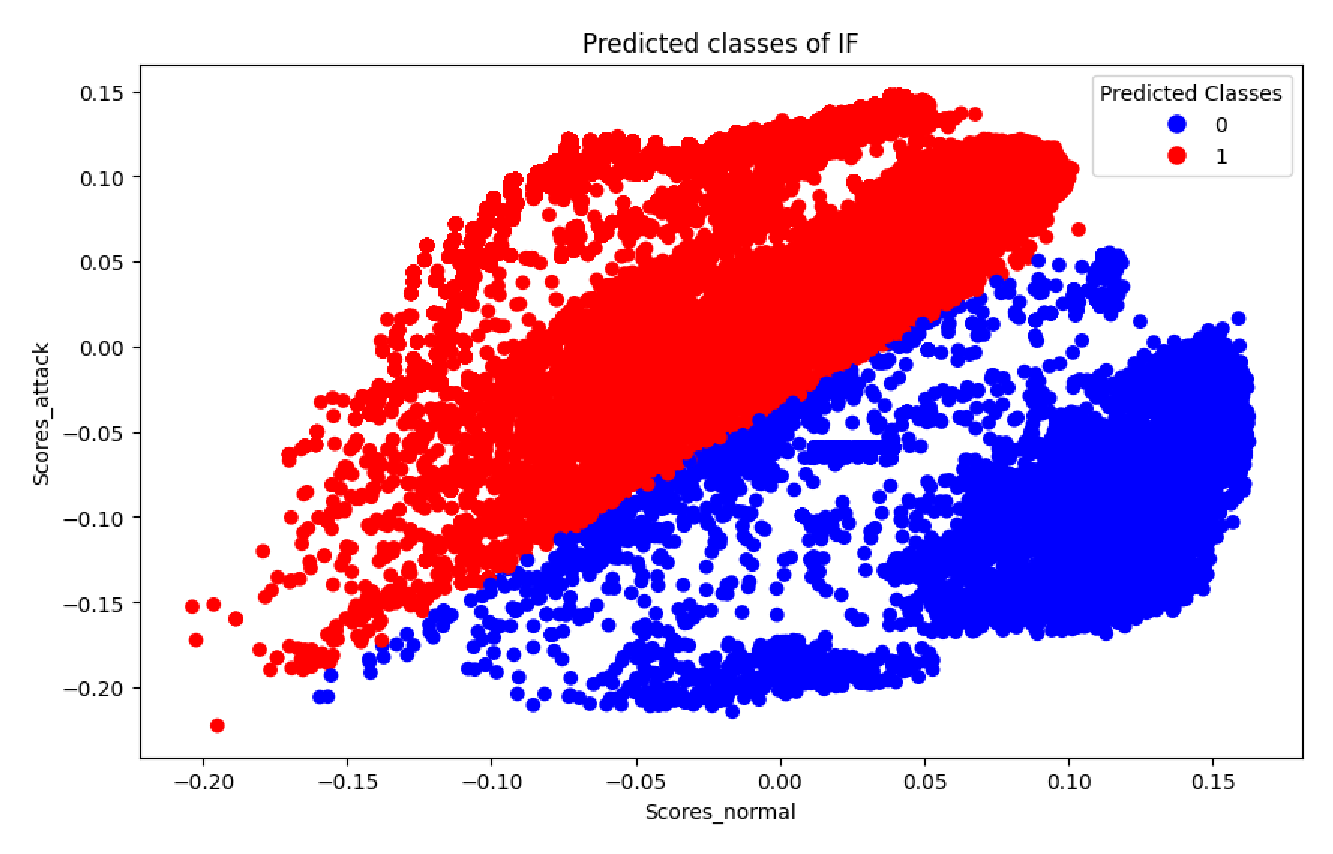
\includegraphics[width=\linewidth]{pictures/eps/UNSW-NB153.eps}
        \caption{UNSW-NB15における提案手法による結果}
        \label{fig:UNSW-NB153}
    \end{minipage}
    \vfill{} 
    \begin{minipage}{0.9\linewidth}
        \centering
        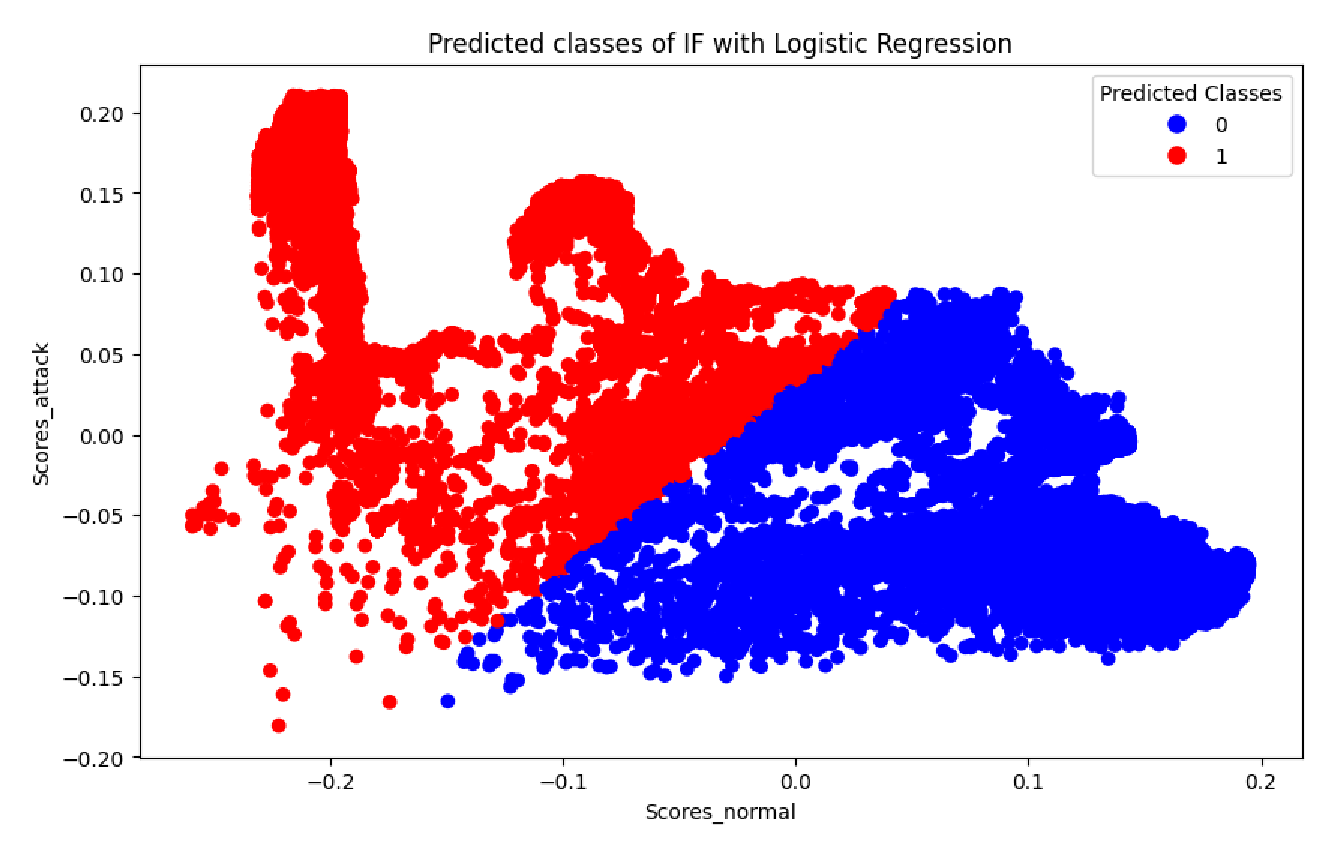
\includegraphics[width=\linewidth]{pictures/eps/NSL-KDD3.eps}
        \caption{NSL-KDDにおける提案手法による結果}
        \label{fig:NSL-KDD3}
    \end{minipage}
\end{figure}

まず, ロジスティック回帰を導入することで, 異常スコアの分布が斜めに広がる場合により正確な境界を引くことが可能になった. 図\ref{fig:UNSW-NB152}と図\ref{fig:NSL-KDD2}はそれぞれ, 2つのサブシステムの判定結果を組み合わせた従来の手法の判定結果を示しており, 図\ref{fig:UNSW-NB153}と図\ref{fig:NSL-KDD3}はロジスティック回帰を用いた提案手法の判定結果を示している. 図\ref{fig:UNSW-NB152}と図\ref{fig:NSL-KDD2}から, 2つのサブシステムの判定を組み合わせた手法において, どれだけ閾値を適切に設定したとしても, 異常スコアの分布が斜めに広がる場合には誤判定が多く発生することがわかる. 一方, 図\ref{fig:UNSW-NB153}と図\ref{fig:NSL-KDD3}からは, ロジスティック回帰を用いた手法が, 斜めに広がる異常スコアの分布に対しても, より正確に判定できることが確認できる. 従来の垂直な分割では誤判定が多発するケースにおいても, 精度の向上が見込めることが実証された. 

また, 本アプローチが適用できる範囲についても考察が必要である. 異常スコアの分布において, 正常な通信と攻撃通信が直線的に分離できている場合, この手法は効果的である. しかし, 攻撃通信と正常な通信が十分に分離されていない場合や, 境界線が曲線状になっている場合には, 判定精度が低くなる可能性がある. 実際, 図\ref{fig:UNSW-NB151}を見ると, 斜めに分布した攻撃通信の中に正常な通信が多く混ざっている. 一方で図\ref{fig:NSL-KDD1}では, 概ね攻撃通信と正常な通信が分離され, お互いが混ざりあう部分が比較的小さい. これら2つのデータセットを比較すると, NSL-KDDはUNSW-NB15よりも高い検知精度を示している. このように, 異常スコアの分布によっては効果的でない場合があり, 別の特徴量選択手法の採用や異なる機械学習アルゴリズムの適用など, さらなる工夫が必要となる可能性がある. 

さらに, ロジスティック回帰を適用する際のコストや計算量に関するトレードオフも存在する. IF単体での異常検知に比べ, ロジスティック回帰を用いることでモデル構築にかかる計算時間が増加することが懸念される. 

以上より, 提案手法は特定の条件下では高い効果を発揮することが確認されたが, 全てのシナリオにおいて有効であるとは限らない. 今後は, 異常スコアの分布がさらに複雑な場合における改良や, 計算効率の最適化について検討することが求められる. 

\section{おわりに}
本研究では, 家庭環境でも高速に動作するようなIDSの提案を目指すため, AbuAlghanamらが提案したIFを用いたIoT環境向けの異常検知手法\cite{AbuAlghanam2023-sx}に注目し, その手法の改善を行なった. AbuAlghanamらの手法には, 手動で閾値を設定する必要がある点や, 判定の組み合わせ方法における精度の限界といった課題が存在していた. これらの課題を解決するためにロジスティック回帰を応用した判定アルゴリズムを導入した. この新しいアルゴリズムにより異常スコアの分布に応じた柔軟な境界設定が可能となり, AbuAlghanamらの判定組み合わせ手法に比べて, 精度が大幅に向上したことが確認された. 今後の課題として, より複雑な異常スコアの分布に対する適用性の検討や計算効率の最適化が求められる. 

\bibliographystyle{ipsjsort} % 参照順
\bibliography{references}

\end{document}
